\section{Fichier DICOM}

\frame
{
	\frametitle{Conventions DICOM}
	\begin{itemize}
		\item Single Frame
		\begin{itemize}
			\item Une image : stock\'ee dans un fichier.
			\item Une coupe = une image
		
			$\Rightarrow$ s\'erie de 100 coupes = 100 fichiers.
		\end{itemize}
		\item Multiframe
		\begin{itemize}
			\item Aussi appel\'e \emph{Enhanced DICOM}.
			\item Plusieurs images dans la m\^eme s\'equence.
			
			E.g. s\'equence vid\'eo d'\'echographie.
		\end{itemize}
		\item Arborescence des r\'epertoires/fichiers
		\begin{center}
			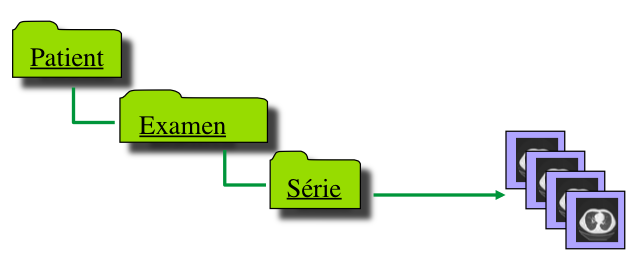
\includegraphics[width=.8\linewidth]{./figures/arborescence.png}
		\end{center}

	\end{itemize}
}

\frame
{
	\frametitle{Fichier en pratique}
	
	\begin{itemize}
		\item Peut \^etre exp\'edi\'e par messagerie.
		\item Convertible en d'autres formats (JPEG, AVI, etc.)
		\item Extenstion : .dcm
		\item Exemple avec OsiriX.
	\end{itemize}
}

\frame
{
	\frametitle{Contenu d'un fichier .dcm}
	
	Un fichier DICOM est l'agr\'egation des \'el\'ements suivants :
	\begin{itemize}
		\item Pr\'e-ent\^ete :
		\begin{itemize}
			\item Pr\'eambule : 128 octets de donn\'ees "application".
			\item Pr\'efixe : 0x4449434D=DICM (4 octets).
		\end{itemize}
		\item Suite de Data Elements.
		En g\'en\'eral :
		\begin{itemize}
			\item Tag ;
			\item VR ;
			\item Taille ;
			\item et Valeur.
		\end{itemize}
	\end{itemize}
}

\frame
{
	\frametitle{Tag}

	Il s'agit de l'\'etiquette d'identification d'un \'el\'ement d'information.
	\begin{itemize}
		\item Identifi\'e par un couple de deux nombres en h\'exad\'ecimal (Group Number, Element Number) :
			\begin{description}
				\item[Group Number] Identifiant d'un ensemble de tags (e.g. Patient, Study,\ldots).
				\item[Element Number] Position de l'\'el\'ement dans son groupe.
			\end{description}
		\item Exemple : l'\'el\'ement \emph{PatientID} a pour tag $(0010,0020)$.
		\item Une liste -- quasi -- exhaustive des tags ($3307$ tags diff\'erents, y compris nombre de tags obsol\`etes) : \url{http://www.dicomtags.com/iods}
		\item Certains tags sont "propri\'etaires", i.e. cr\'e\'es et utilis\'es par un constructeur particulier.
	\end{itemize}
}

\frame
{
	\frametitle{Value Representation}

	\begin{itemize}
		\item Tous les \'el\'ements ne sont pas repr\'esent\'es par le m\^eme type de donn\'ees.
		\item Donn\'ee num\'erique $\neq$ Donn\'ee textuelle.
		\item Ensemble des VR : \url{http://www.dicomtags.com/vrs}
	\end{itemize}
}

